\documentclass[aspectratio=169,11pt]{beamer}

\usepackage[utf8]{inputenc}
\usepackage[T5]{fontenc}
\usepackage[vietnamese]{babel}
\usepackage{graphicx}
\usepackage{booktabs}
\usepackage{array}
\usepackage{amsmath}
\usepackage{tikz}
\usepackage{pgfplots}
\usetikzlibrary{arrows.meta,positioning,fit,calc,shapes.geometric}
\pgfplotsset{compat=1.18}
\graphicspath{{images/}}

\usetheme{Madrid}
\usecolortheme{default}
\setbeamertemplate{navigation symbols}{}
\setbeamertemplate{footline}[frame number]
\setbeamerfont{frametitle}{series=\bfseries,size=\large}
\setbeamerfont{title}{series=\bfseries,size=\Large}

\definecolor{bkblue}{RGB}{24,79,141}
\definecolor{softblue}{RGB}{232,241,250}
\definecolor{softorange}{RGB}{252,239,221}
\definecolor{softgreen}{RGB}{231,246,235}
\definecolor{softred}{RGB}{252,231,231}
\setbeamercolor{structure}{fg=bkblue}
\setbeamercolor{frametitle}{fg=bkblue}

\newcommand{\metriccard}[3]{%
  \begin{tikzpicture}
    \node[draw=bkblue!40, rounded corners=4pt, fill=#1, text width=0.9\linewidth, minimum height=1.4cm, align=center] {
      \textbf{#2}\\[0.25em]
      {\small #3}
    };
  \end{tikzpicture}%
}

\title{Phát triển Marketing Agent cho SME ngành F\&B}
\subtitle{Đề án tốt nghiệp}
\author{Võ Quang Nhân}
\institute{Trường Đại học Bách Khoa -- ĐHQG TP.HCM}
\date{Tháng 05/2026}

\begin{document}

\begin{frame}[plain]
  \titlepage
  \vfill
  \begin{center}
    {\small GVHD: TS. Nguyễn An Khương}
  \end{center}
\end{frame}

\begin{frame}{Bối cảnh và động cơ nghiên cứu}
  \begin{columns}[T,onlytextwidth]
    \begin{column}{0.42\textwidth}
      \begin{block}{SME F\&B}
        Phụ thuộc Facebook để duy trì hiện diện thương hiệu, nhưng thiếu nguồn lực sản xuất nội dung đều đặn.
      \end{block}
      \begin{block}{Khoảng trống}
        Công cụ AI tổng quát chưa nắm tốt ngữ cảnh địa phương, đặc trưng ngành và giọng thương hiệu.
      \end{block}
    \end{column}
    \begin{column}{0.54\textwidth}
      \centering
      \begin{tikzpicture}[scale=0.86, transform shape, node distance=1.0cm, every node/.style={font=\small}]
        \node[draw, rounded corners, fill=softblue, minimum width=4.4cm, minimum height=1cm] (need) {Nhu cầu nội dung ổn định};
        \node[draw, rounded corners, fill=softorange, below=of need, minimum width=4.4cm, minimum height=1cm] (cost) {Chi phí và nhân lực hạn chế};
        \node[draw, rounded corners, fill=softred, below=of cost, minimum width=4.4cm, minimum height=1cm] (generic) {AI tổng quát chưa chuyên biệt};
        \node[draw, rounded corners, fill=softgreen, right=1.2cm of cost, minimum width=3.2cm, minimum height=2.2cm, align=center] (goal) {\textbf{Marketing Agent}\\chuyên biệt F\&B};
        \draw[-{Stealth}] (need.east) -- (goal.north west);
        \draw[-{Stealth}] (cost.east) -- (goal.west);
        \draw[-{Stealth}] (generic.east) -- (goal.south west);
      \end{tikzpicture}
    \end{column}
  \end{columns}
\end{frame}

\begin{frame}[t]{Bài toán: Brief vào -- bài đăng ra -- đạt ngưỡng chất lượng}
  \vspace{0.5cm}
  \centering
  \begin{tikzpicture}[node distance=0.7cm, every node/.style={font=\small}]
    \node[draw, rounded corners, fill=softblue,
          text width=2.6cm, minimum height=2.2cm, align=center] (input)
      {\textbf{Đầu vào}\\[0.4em]
       {\footnotesize Sản phẩm, brief chiến dịch, phong cách thương hiệu}};
    \node[draw, rounded corners, fill=softgreen,
          right=0.7cm of input, text width=2.6cm, minimum height=2.2cm, align=center] (agent)
      {\textbf{Marketing Agent}\\[0.4em]
       {\footnotesize AI sinh nội dung chuyên biệt F\&B}};
    \node[draw, rounded corners, fill=softorange,
          right=0.7cm of agent, text width=2.6cm, minimum height=2.2cm, align=center] (output)
      {\textbf{Bài đăng}\\[0.4em]
       {\footnotesize Caption + ảnh minh họa Facebook}};
    \node[draw, rounded corners, fill=softred,
          right=0.7cm of output, text width=2.6cm, minimum height=2.2cm, align=center] (eval)
      {\textbf{Kiểm duyệt}\\[0.4em]
       {\footnotesize Đạt đủ 3 tiêu chí F, E, V mới chấp nhận}};
    \draw[-{Stealth}, thick] (input)  -- (agent);
    \draw[-{Stealth}, thick] (agent)  -- (output);
    \draw[-{Stealth}, thick] (output) -- (eval);
  \end{tikzpicture}

  \vspace{0.6cm}
  \begin{columns}[T,onlytextwidth]
    \begin{column}{0.32\textwidth}
      \centering\metriccard{softblue}{F -- Faithfulness}{Nội dung trung thực với brief, không bịa thêm}
    \end{column}
    \begin{column}{0.32\textwidth}
      \centering\metriccard{softorange}{E -- Expansion}{Thông tin được mở rộng tự nhiên, hấp dẫn}
    \end{column}
    \begin{column}{0.32\textwidth}
      \centering\metriccard{softgreen}{V -- Vibe}{Giọng văn phù hợp phong cách thương hiệu}
    \end{column}
  \end{columns}
\end{frame}

\begin{frame}[t]{Câu hỏi nghiên cứu, mục tiêu và phạm vi}
  \begin{columns}[T,onlytextwidth]
    \begin{column}{0.55\textwidth}
      \begin{enumerate}
        \item Có thể xây dựng Marketing Agent $\pi_\theta$ chuyên biệt cho SME F\&B không?
        \item Có thể đánh giá bằng $\text{Overall}=\tfrac{1}{3}(F+E+V)$ tự động không?
        \item SFT và RL ảnh hưởng thế nào đến $\mathbb{E}[\text{Overall}]$ trên tập thực tế?
      \end{enumerate}
    \end{column}
    \begin{column}{0.41\textwidth}
      \begin{block}{Phạm vi}
        \begin{itemize}
          \item Nội dung Facebook, SME F\&B, tiếng Việt
          \item Có bước phê duyệt: $\text{Overall} \geq \theta$
          \item Thực nghiệm: $n=100$ trường hợp F\&B
        \end{itemize}
      \end{block}
      \begin{block}{Liên kết RQ}
        RQ1: $x \to y$;\; RQ2: $\text{Overall}$;\; RQ3: $\Delta$ sau SFT/GRPO.
      \end{block}
    \end{column}
  \end{columns}
  \vspace{0.4em}
  \centering
  \begin{tikzpicture}[every node/.style={font=\small}]
    \node[draw, rounded corners, fill=softblue, minimum width=3.0cm, minimum height=1.0cm] (system) {Hệ thống $\pi_\theta$};
    \node[draw, rounded corners, fill=softgreen, right=0.8cm of system, minimum width=3.0cm, minimum height=1.0cm] (eval) {Đánh giá $F/E/V$};
    \node[draw, rounded corners, fill=softorange, right=0.8cm of eval, minimum width=3.0cm, minimum height=1.0cm] (learning) {Huấn luyện SFT/GRPO};
    \draw[-{Stealth}, thick] (system) -- (eval);
    \draw[-{Stealth}, thick] (eval) -- (learning);
  \end{tikzpicture}
\end{frame}

\begin{frame}{Tổng quan đóng góp và phương pháp}
  \centering
  \begin{tikzpicture}[node distance=1.1cm, every node/.style={font=\small}]
    \node[draw, rounded corners, fill=softblue, text width=3.2cm, minimum height=2.1cm, align=center] (system) {
      \textbf{System}\\
      Multi-agent LangGraph\\
      Campaign -- Content -- Image
    };
    \node[draw, rounded corners, fill=softgreen, right=of system, text width=3.2cm, minimum height=2.1cm, align=center] (evaluation) {
      \textbf{Evaluation}\\
      Faithfulness\\
      Expansion\\
      Vibe
    };
    \node[draw, rounded corners, fill=softorange, right=of evaluation, text width=3.2cm, minimum height=2.1cm, align=center] (learning) {
      \textbf{Learning Loop}\\
      SFT / GRPO\\
      Preference về sau
    };
    \draw[-{Stealth}, thick] (system) -- (evaluation);
    \draw[-{Stealth}, thick] (evaluation) -- (learning);
    \draw[-{Stealth}, thick, bend left=25] (learning.north) to node[above]{\scriptsize cải thiện} (system.north);
  \end{tikzpicture}

  \vspace{1.0em}
  \begin{block}{Luận điểm chính}
    Đề án không chỉ xây hệ thống sinh nội dung, mà còn xây khung đánh giá và chỉ ra điều kiện dữ liệu cần có để tối ưu RL đúng về sau.
  \end{block}
\end{frame}

\begin{frame}[t]{Cơ sở lý thuyết cần thiết}
  \begin{columns}[T,onlytextwidth]
    \begin{column}{0.34\textwidth}
      \metriccard{softblue}{LLM / Qwen3.5}{Sinh văn bản theo ngữ cảnh, phù hợp thử nghiệm mô hình mở}
    \end{column}
    \begin{column}{0.34\textwidth}
      \metriccard{softgreen}{SFT / QLoRA}{Học từ cặp input-output đã kiểm duyệt với chi phí thấp}
    \end{column}
    \begin{column}{0.28\textwidth}
      \metriccard{softorange}{RL Alignment}{RLHF, DPO, GRPO phụ thuộc tín hiệu preference/reward}
    \end{column}
  \end{columns}

  \vspace{0.6em}
  \centering
  \begin{tikzpicture}[node distance=1cm, every node/.style={font=\small}]
    \node[draw, rounded corners, fill=softblue, minimum width=2.3cm] (base) {Base LLM};
    \node[draw, rounded corners, fill=softgreen, right=of base, minimum width=2.3cm] (sft) {SFT};
    \node[draw, rounded corners, fill=softorange, right=of sft, minimum width=2.5cm] (pref) {Preference};
    \node[draw, rounded corners, fill=softred, right=of pref, minimum width=2.1cm] (rl) {RL/DPO};
    \draw[-{Stealth}, thick] (base) -- (sft);
    \draw[-{Stealth}, thick] (sft) -- (pref);
    \draw[-{Stealth}, thick] (pref) -- (rl);
  \end{tikzpicture}

  \eqblock{%
    \begin{align*}
      \mathcal{L}_{\text{SFT}} &= -\mathbb{E}_{(x,y^*)}\bigl[\log \pi_\theta(y^* \mid x)\bigr],\\
      W &= W_0 + BA,\quad B \in \mathbb{R}^{d_{\mathrm{out}}\times r},\;
      A \in \mathbb{R}^{r\times d_{\mathrm{in}}},\; r \ll d,\\
      \hat{A}_i &= \dfrac{r_i - \mathrm{mean}(r)}{\mathrm{std}(r)} \quad \text{(GRPO)}
    \end{align*}%
  }
\end{frame}

\begin{frame}[t]{Kiến trúc hệ thống Marketing Agent}
  \begin{columns}[T,onlytextwidth]
    \begin{column}{0.68\textwidth}
      \centering
      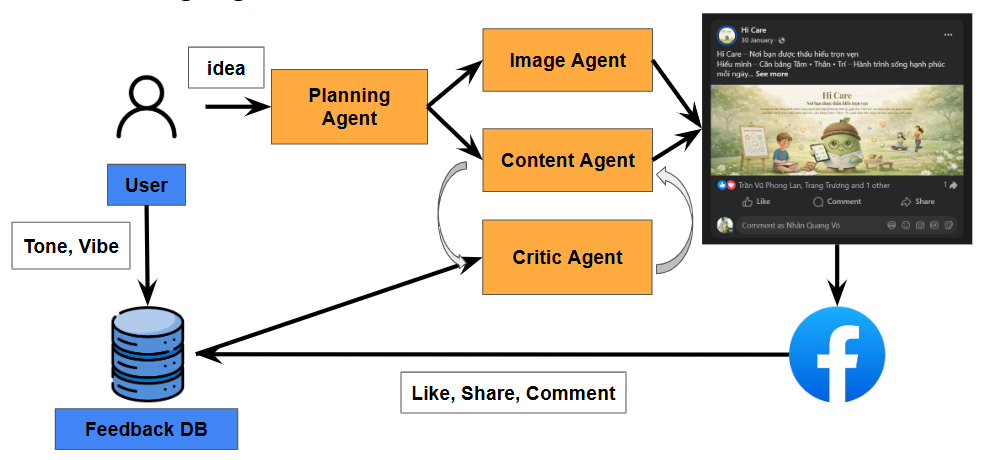
\includegraphics[width=\linewidth,height=0.78\textheight,keepaspectratio]{system_architecture.png}
    \end{column}
    \begin{column}{0.30\textwidth}
      \begin{block}{Agent \& luồng}
        $x \!\to\! plan \!\to\! y \!\to\! img$\\
        Campaign, Content, Image agents
      \end{block}
      \begin{block}{Hạ tầng \& đánh giá}
        FastAPI, PostgreSQL, Celery, MinIO\\
        $F,E,V$; duyệt nếu $\text{Overall}\geq\theta$
      \end{block}
    \end{column}
  \end{columns}
\end{frame}

\begin{frame}{Luồng xử lý nghiệp vụ và phê duyệt}
  \centering
  \begin{tikzpicture}[
    node distance=0.55cm,
    every node/.style={font=\small},
    stepbox/.style={draw, rounded corners, fill=softblue, text width=2.15cm, minimum height=1.1cm, align=center}
  ]
    \node[stepbox] (brief) {Campaign\\brief};
    \node[stepbox, fill=softgreen, right=of brief] (plan) {Content\\plan};
    \node[stepbox, fill=softorange, right=of plan] (gen) {Generate\\content};
    \node[stepbox, fill=softblue, right=of gen] (eval) {Evaluate\\F/E/V};
    \node[stepbox, fill=softred, right=of eval] (human) {Human\\approval};

    \draw[-{Stealth}, thick] (brief) -- (plan);
    \draw[-{Stealth}, thick] (plan) -- (gen);
    \draw[-{Stealth}, thick] (gen) -- (eval);
    \draw[-{Stealth}, thick] (eval) -- (human);

    \node[stepbox, fill=softgreen, below=1.2cm of gen, text width=3.1cm] (store) {Store feedback\\for continuous improvement};
    \draw[-{Stealth}, thick] (human.south) |- (store.east);
    \draw[-{Stealth}, thick, dashed] (store.west) -| (plan.south);
  \end{tikzpicture}

  \vspace{1em}
  \begin{alertblock}{Nguyên tắc vận hành}
    Tự động hóa phần sinh và đánh giá, nhưng người dùng vẫn giữ quyền quyết định trước khi sản xuất hàng loạt.
  \end{alertblock}
\end{frame}

\begin{frame}[t]{Đánh giá tự động ba chiều: Faithfulness, Expansion \& Marketing Vibe}
  \centering
  \vspace{0.1cm}
  \begin{tikzpicture}[every node/.style={font=\small}]

    % ---- Cột 1: Overall ----
    \node[draw, rounded corners, fill=softred, text width=2.3cm,
          minimum height=6.6cm, align=center, font=\normalsize] (overall) at (0, -0.5) {
      \textbf{Overall}\\[5pt]
      $\dfrac{F+E+V}{3}$\\[5pt]
      $\theta=0{,}75$
    };

    % ---- Cột 2: Metrics ----
    \node[draw, rounded corners, fill=softblue, text width=3.3cm,
          minimum height=2.1cm, align=center] (faith) at (4.5, 1.7) {
      \textbf{Faithfulness}\\[5pt]
      $F=0{,}5\,s_r+0{,}5\,s_l$
    };
    \node[draw, rounded corners, fill=softgreen, text width=3.3cm,
          minimum height=2.1cm, align=center] (exp) at (4.5, -0.5) {
      \textbf{Expansion}\\[5pt]
      $E=0{,}9\,s_l+0{,}1\,s_r$
    };
    \node[draw, rounded corners, fill=softorange, text width=3.3cm,
          minimum height=2.1cm, align=center] (vibe) at (4.5, -2.7) {
      \textbf{Marketing Vibe}\\[5pt]
      $V=\mathrm{clip}(0{,}85\,s_V+0{,}15\,s_f-p)$
    };

    % ---- Cột 3: Sub-components (spacing 1.1cm center-to-center) ----
    \node[draw, rounded corners, fill=softblue!30, text width=4.0cm,
          minimum height=0.9cm, align=center, font=\scriptsize] (f_rule) at (9.5, 2.25) {
      \textbf{EntityPresenceRule}\\
      regex: giá, spec, combo, tên
    };
    \node[draw, rounded corners, fill=softblue!30, text width=4.0cm,
          minimum height=0.9cm, align=center, font=\scriptsize] (f_llm) at (9.5, 1.15) {
      \textbf{GEval Faithfulness}\\
      LLM: kiểm claim vô căn cứ
    };
    \node[draw, rounded corners, fill=softgreen!30, text width=4.0cm,
          minimum height=0.9cm, align=center, font=\scriptsize] (e_rule) at (9.5, 0.05) {
      \textbf{ContentExpansionRule}\\
      length, benefit, context
    };
    \node[draw, rounded corners, fill=softgreen!30, text width=4.0cm,
          minimum height=0.9cm, align=center, font=\scriptsize] (e_llm) at (9.5, -1.05) {
      \textbf{GEval Expansion}\\
      LLM: diễn giải lợi ích
    };
    \node[draw, rounded corners, fill=softorange!30, text width=4.0cm,
          minimum height=0.9cm, align=center, font=\scriptsize] (v_rule) at (9.5, -2.15) {
      \textbf{FbStructureRule + Penalty}\\
      đoạn ngắn, CTA, hype penalty
    };
    \node[draw, rounded corners, fill=softorange!30, text width=4.0cm,
          minimum height=0.9cm, align=center, font=\scriptsize] (v_llm) at (9.5, -3.25) {
      \textbf{VibeJudge D1--D5}\\
      Voice·Biz·Persuasion·CTA·FB
    };

    % ---- Mũi tên: sub-components → metrics ----
    \draw[-{Stealth}] (f_rule.west) -- (faith.east |- f_rule);
    \draw[-{Stealth}] (f_llm.west)  -- (faith.east |- f_llm);
    \draw[-{Stealth}] (e_rule.west) -- (exp.east |- e_rule);
    \draw[-{Stealth}] (e_llm.west)  -- (exp.east |- e_llm);
    \draw[-{Stealth}] (v_rule.west) -- (vibe.east |- v_rule);
    \draw[-{Stealth}] (v_llm.west)  -- (vibe.east |- v_llm);

    % ---- Mũi tên: metrics → overall ----
    \draw[-{Stealth}] (faith.west) -- (overall.east |- faith);
    \draw[-{Stealth}] (exp.west)   -- (overall.east);
    \draw[-{Stealth}] (vibe.west)  -- (overall.east |- vibe);

  \end{tikzpicture}
\end{frame}

\begin{frame}{Thiết kế thực nghiệm}
  \centering
  \begin{tikzpicture}[
    node distance=0.9cm,
    every node/.style={font=\small},
    box/.style={draw, rounded corners, text width=3.0cm, minimum height=1.3cm, align=center}
  ]
    \node[box, fill=softblue] (base) {\textbf{Baseline}\\Qwen3.5 2B, 4B, 9B};
    \node[box, fill=softgreen, right=of base] (sft) {\textbf{SFT / QLoRA}\\Qwen3.5 2B, 4B};
    \node[box, fill=softorange, right=of sft] (grpo) {\textbf{GRPO}\\Qwen3.5 2B\\reward rule-based};
    \node[box, fill=softred, below=1.2cm of sft] (eval) {\textbf{Evaluation}\\100 trường hợp F\&B\\F/E/V + Overall};

    \draw[-{Stealth}, thick] (base) -- (sft);
    \draw[-{Stealth}, thick] (sft) -- (grpo);
    \draw[-{Stealth}, thick] (base.south) -- (eval.north west);
    \draw[-{Stealth}, thick] (sft.south) -- (eval.north);
    \draw[-{Stealth}, thick] (grpo.south) -- (eval.north east);
  \end{tikzpicture}

  \vspace{1em}
  \begin{block}{Mục tiêu thực nghiệm}
    Đo tác động của tinh chỉnh có giám sát và học tăng cường đối với chất lượng nội dung marketing F\&B tiếng Việt.
  \end{block}
\end{frame}

\begin{frame}{Kết quả thực nghiệm chính}
  \begin{columns}[T,onlytextwidth]
    \begin{column}{0.66\textwidth}
      \centering
      \begin{tikzpicture}
        \begin{axis}[
          ybar,
          ymin=0,
          ymax=0.8,
          width=\linewidth,
          height=0.64\textheight,
          bar width=14pt,
          symbolic x coords={2B,4B,4B+SFT,GPT},
          xtick=data,
          ylabel={Overall},
          nodes near coords,
          nodes near coords style={font=\scriptsize},
          every axis plot/.append style={fill=bkblue!65},
          tick label style={font=\scriptsize},
          label style={font=\small}
        ]
          \addplot coordinates {(2B,0.570) (4B,0.622) (4B+SFT,0.687) (GPT,0.707)};
        \end{axis}
      \end{tikzpicture}
    \end{column}
    \begin{column}{0.31\textwidth}
      \begin{block}{Kết quả nổi bật}
        \begin{itemize}
          \item 4B + SFT đạt 0,687 Overall
          \item GPT-5.4-mini đạt 0,707
          \item Chênh lệch khoảng 2,8\%
        \end{itemize}
      \end{block}
      \begin{alertblock}{Điểm đáng chú ý}
        Vibe của 4B + SFT tương đương mô hình thương mại.
      \end{alertblock}
    \end{column}
  \end{columns}
\end{frame}

\begin{frame}{Vai trò của SFT trong hệ thống}
  \centering
  \begin{tikzpicture}[
    node distance=1.2cm,
    every node/.style={font=\small},
    box/.style={draw, rounded corners, text width=3.1cm, minimum height=1.4cm, align=center}
  ]
    \node[box, fill=softblue] (before) {\textbf{Before SFT}\\Phụ thuộc nhiều vào prompt\\giọng văn chưa ổn định};
    \node[box, fill=softgreen, right=of before] (sft) {\textbf{SFT}\\Học từ dữ liệu F\&B\\đã kiểm duyệt};
    \node[box, fill=softorange, right=of sft] (after) {\textbf{Candidate Generator}\\Sinh nhiều phương án\\cho cùng một brief};
    \draw[-{Stealth}, thick] (before) -- (sft);
    \draw[-{Stealth}, thick] (sft) -- (after);
  \end{tikzpicture}

  \vspace{1.2em}
  \begin{block}{Thông điệp}
    SFT không phải điểm dừng cuối, mà là bước nền để tạo các ứng viên đủ tốt cho thu thập preference hợp lệ.
  \end{block}
\end{frame}

\begin{frame}[t]{Dữ liệu huấn luyện: GRPO vs DPO}
  \begin{columns}[T,onlytextwidth]
    \begin{column}{0.48\textwidth}
      \textbf{\color{bkblue}GRPO --- Verifiable Reward}
      \begin{itemize}\small
        \item Prompt $x$ + nhiều output $\{y_i\}_{i=1}^G$
        \item Scalar reward $r_i \in \{0,1\}$ kiểm chứng tự động
        \item Phù hợp: code, toán học, logic
      \end{itemize}
      \vspace{0.5em}
      \scriptsize
      \textit{Ví dụ: bài toán có đáp án đúng/sai rõ ràng}
    \end{column}
    \begin{column}{0.48\textwidth}
      \textbf{\color{orange}DPO --- Preference Pairs}
      \begin{itemize}\small
        \item Cặp $(x,\, y^+,\, y^-)$ cùng prompt
        \item $y^+$ được ưa thích hơn $y^-$ (human label)
        \item Phù hợp: marketing, sáng tạo nội dung
      \end{itemize}
      \vspace{0.5em}
      \scriptsize
      \textit{Ví dụ: annotator chọn bài viết hay hơn}
    \end{column}
  \end{columns}

  \vspace{0.5em}
  \begin{block}{Tại sao không dùng GRPO cho marketing?}
    \scriptsize
    GRPO yêu cầu reward $r_i$ có phương sai đủ lớn trong nhóm $G$ cùng prompt.
    Chất lượng text marketing không có verifiable reward $\Rightarrow$ không thỏa mãn điều kiện này.
    DPO tối ưu trực tiếp từ cặp $(x, y^+, y^-)$ \textbf{mà không cần scalar reward}.
  \end{block}

  \eqblock{%
    GRPO: $A_i = (r_i - \bar{r})/\sigma_r$, cần $r_i$ verifiable \quad
    DPO: $\mathcal{L}_{\text{DPO}} \propto -\log\sigma(\beta\,\Delta\log\pi)$, chỉ cần $(y^+, y^-)$
  }
\end{frame}

\begin{frame}{Vì sao post rời rạc không đủ cho reward model}
  \centering
  \begin{tikzpicture}[
    node distance=0.75cm,
    every node/.style={font=\small},
    box/.style={draw, rounded corners, text width=2.5cm, minimum height=1cm, align=center}
  ]
    \node[box, fill=softblue] (pa) {Prompt A};
    \node[box, fill=softgreen, right=1cm of pa] (oa) {Post A\\score cao};
    \node[box, fill=softblue, below=1.2cm of pa] (pb) {Prompt B};
    \node[box, fill=softorange, right=1cm of pb] (ob) {Post B\\score thấp};
    \node[box, fill=softred, right=1.3cm of oa, yshift=-0.6cm, text width=3.2cm, minimum height=2.2cm] (wrong) {\textbf{Ghép sai}\\Post A = chosen\\Post B = rejected};

    \draw[-{Stealth}, thick] (pa) -- (oa);
    \draw[-{Stealth}, thick] (pb) -- (ob);
    \draw[-{Stealth}, thick, dashed] (oa) -- (wrong);
    \draw[-{Stealth}, thick, dashed] (ob) -- (wrong);
  \end{tikzpicture}

  \vspace{1em}
  \begin{alertblock}{Vấn đề lý thuyết}
    Chosen/rejected chỉ có ý nghĩa khi hai output cùng xuất phát từ một prompt. Ghép hai post khác prompt khiến reward model học tương quan giả.
  \end{alertblock}
\end{frame}

\begin{frame}[t]{Vì sao engagement reward không scalable}
  \begin{columns}[T,onlytextwidth]
    \begin{column}{0.48\textwidth}
      \centering
      \begin{tikzpicture}[node distance=0.85cm, every node/.style={font=\small}]
        \node[draw, rounded corners, fill=softgreen, text width=3.8cm, align=center] (task) {Code / Toán};
        \node[draw, rounded corners, fill=softgreen, below=of task, text width=3.8cm, align=center] (verify) {Verifier tức thì\\test case / đáp án};
        \node[draw, rounded corners, fill=softgreen, below=of verify, text width=3.8cm, align=center] (reward) {Reward rõ ràng};
        \draw[-{Stealth}, thick] (task) -- (verify);
        \draw[-{Stealth}, thick] (verify) -- (reward);
      \end{tikzpicture}
    \end{column}
    \begin{column}{0.48\textwidth}
      \centering
      \begin{tikzpicture}[node distance=0.85cm, every node/.style={font=\small}]
        \node[draw, rounded corners, fill=softorange, text width=3.8cm, align=center] (content) {Marketing content};
        \node[draw, rounded corners, fill=softorange, below=of content, text width=3.8cm, align=center] (publish) {Phải đăng lên Facebook};
        \node[draw, rounded corners, fill=softred, below=of publish, text width=3.8cm, align=center] (risk) {Chậm, nhiễu, rủi ro kinh doanh};
        \draw[-{Stealth}, thick] (content) -- (publish);
        \draw[-{Stealth}, thick] (publish) -- (risk);
      \end{tikzpicture}
    \end{column}
  \end{columns}

  \eqblock{%
    \begin{align*}
      e_{\text{raw}} &= L + 0{,}5C + 1{,}5S + R_{\text{like}} + 1{,}2 R_{\text{love}}
      + 0{,}8(R_{\text{haha}}+R_{\text{care}}+R_{\text{wow}}) - 0{,}5 R_{\text{angry}} - 0{,}3 R_{\text{sad}}\\
      e &= \ln(1 + \max(e_{\text{raw}}, 0)),\quad
      \max_\theta \mathbb{E}[r] \not\approx \max_\theta \mathbb{E}[\text{Overall}] \;\text{(SME)}
    \end{align*}
  }
\end{frame}

\begin{frame}{Phân tích thất bại GRPO và bài học}
  \begin{columns}[T,onlytextwidth]
    \begin{column}{0.62\textwidth}
      \centering
      \begin{tikzpicture}
        \begin{axis}[
          ybar,
          ymin=0,
          ymax=0.65,
          width=\linewidth,
          height=0.62\textheight,
          bar width=18pt,
          symbolic x coords={Baseline,GRPO},
          xtick=data,
          ylabel={Overall},
          nodes near coords,
          nodes near coords style={font=\scriptsize},
          tick label style={font=\scriptsize},
          every axis plot/.append style={fill=softred, draw=bkblue}
        ]
          \addplot coordinates {(Baseline,0.570) (GRPO,0.352)};
        \end{axis}
      \end{tikzpicture}
    \end{column}
    \begin{column}{0.34\textwidth}
      \begin{alertblock}{Reward mismatch}
        Reward chủ yếu đo độ khớp hoặc trung thực với dữ liệu mẫu, không chứa đủ tín hiệu tương tác thật.
      \end{alertblock}
      \begin{block}{Kết quả}
        Overall giảm 38,2\%, Faithfulness giảm 42,1\%.
      \end{block}
    \end{column}
  \end{columns}
\end{frame}

\begin{frame}{Hướng tiếp cận khả thi: SFT trước, preference sau}
  \centering
  \begin{tikzpicture}[
    node distance=0.75cm,
    every node/.style={font=\small},
    box/.style={draw, rounded corners, minimum height=1cm, align=center}
  ]
    \node[box, fill=softblue, text width=2.5cm] (prompt) {Cùng campaign brief};
    \node[box, fill=softgreen, right=1cm of prompt, text width=2.2cm, yshift=0.75cm] (a) {Output A};
    \node[box, fill=softorange, right=1cm of prompt, text width=2.2cm, yshift=-0.75cm] (b) {Output B};
    \node[box, fill=softred, right=1.1cm of a, yshift=-0.75cm, text width=2.6cm] (human) {Human\\preference};
    \node[box, fill=softblue, right=1.1cm of human, text width=2.7cm] (dataset) {Preference\\dataset};
    \node[box, fill=softgreen, below=1cm of dataset, text width=2.7cm] (train) {Reward model\\DPO / RL};

    \draw[-{Stealth}, thick] (prompt) -- (a);
    \draw[-{Stealth}, thick] (prompt) -- (b);
    \draw[-{Stealth}, thick] (a) -- (human);
    \draw[-{Stealth}, thick] (b) -- (human);
    \draw[-{Stealth}, thick] (human) -- (dataset);
    \draw[-{Stealth}, thick] (dataset) -- (train);
  \end{tikzpicture}

  \vspace{1em}
  \begin{block}{Lợi ích}
    Cặp chosen/rejected cùng prompt được tạo từ thao tác duyệt bài tự nhiên, không cần đăng thử nội dung lên Facebook.
  \end{block}
\end{frame}

\begin{frame}{Đóng góp của đề tài}
  \centering
  \begin{tikzpicture}[node distance=1cm, every node/.style={font=\small}]
    \node[draw, rounded corners, fill=softblue, text width=3.2cm, minimum height=2.2cm, align=center] (c1) {
      \textbf{Kiến trúc}\\
      Multi-agent chuyên biệt cho marketing F\&B
    };
    \node[draw, rounded corners, fill=softgreen, right=of c1, text width=3.2cm, minimum height=2.2cm, align=center] (c2) {
      \textbf{Đánh giá}\\
      Faithfulness, Expansion, Vibe
    };
    \node[draw, rounded corners, fill=softorange, right=of c2, text width=3.2cm, minimum height=2.2cm, align=center] (c3) {
      \textbf{Thực nghiệm}\\
      SFT/GRPO và bài học preference
    };
  \end{tikzpicture}

  \vspace{1em}
  \begin{block}{Đóng góp quy trình}
    Dữ liệu duyệt bài trong vận hành có thể trở thành nguồn preference hợp lệ cho vòng cải thiện liên tục.
  \end{block}
\end{frame}

\begin{frame}[t]{Kết luận}
  \centering
  \vspace{0.3cm}
  \begin{tikzpicture}[node distance=0.75cm, every node/.style={font=\small}]
    \node[draw, rounded corners, fill=softblue, text width=9.6cm, minimum height=1.2cm, align=center] (k1) {
      \textbf{RQ\,1 --} Kiến trúc đa tác nhân chuyên biệt F\&B hoạt động được với SME Việt Nam.
    };
    \node[draw, rounded corners, fill=softgreen, below=of k1, text width=9.6cm, minimum height=1.2cm, align=center] (k2) {
      \textbf{RQ\,2 --} SFT+DPO đạt Overall $0{,}687$ (GPT $0{,}707$, $\Delta{=}{-}2{,}8\%$);
      GRPO chéo miền làm giảm chất lượng $-38{,}2\%$.
    };
    \node[draw, rounded corners, fill=softorange, below=of k2, text width=9.6cm, minimum height=1.2cm, align=center] (k3) {
      \textbf{RQ\,3 --} Bộ tiêu chí F/E/V kết hợp rule-based và LLM Judge là pipeline
      đánh giá tự động khả dụng cho nội dung F\&B tiếng Việt.
    };
  \end{tikzpicture}

  \vspace{0.55cm}
  {\small\itshape SLM 4B sau SFT có thể cạnh tranh API thương mại trong bài toán ngách ---
  mở ra hướng triển khai on-premise, tiết kiệm chi phí cho SME.}
\end{frame}

\begin{frame}{Kết luận}
  \centering
  \begin{tikzpicture}[node distance=0.65cm, every node/.style={font=\small}]
    \node[draw, rounded corners, fill=softblue, text width=8.5cm, minimum height=0.95cm, align=center] (k1) {
      \textbf{1.} Marketing Agent có thể chuyên biệt hóa cho SME F\&B bằng kiến trúc đa tác nhân.
    };
    \node[draw, rounded corners, fill=softgreen, below=of k1, text width=8.5cm, minimum height=0.95cm, align=center] (k2) {
      \textbf{2.} Pipeline F/E/V giúp đo lường chất lượng nội dung và so sánh mô hình một cách nhất quán.
    };
    \node[draw, rounded corners, fill=softorange, below=of k2, text width=8.5cm, minimum height=0.95cm, align=center] (k3) {
      \textbf{3.} Muốn tối ưu RL đúng cần dữ liệu preference cùng prompt, không chỉ engagement rời rạc.
    };
  \end{tikzpicture}

  \vspace{0.55em}
  \begin{block}{Thông điệp cuối}
    SLM mã nguồn mở sau tinh chỉnh có tiềm năng thay thế một phần API thương mại trong bài toán hẹp, nếu được đặt trong vòng đánh giá và thu thập preference phù hợp.
  \end{block}
\end{frame}


\end{document}
